% *********************************************************************
% © 2026 Jeremy Sylvestre
%
% Permission is granted to copy, distribute and/or modify this document
% under the terms of the GNU Free Documentation License, Version 1.3 or
% any later version published by the Free Software Foundation; with no
% Invariant Sections, no Front-Cover Texts, and no Back-Cover Texts. A
% copy of the license is included in the appendix entitled “GNU Free
% Documentation License” that appears in the output document of this
% PreTeXt source code. All trademarks™ are the registered® marks of
% their respective owners.
%
% *********************************************************************
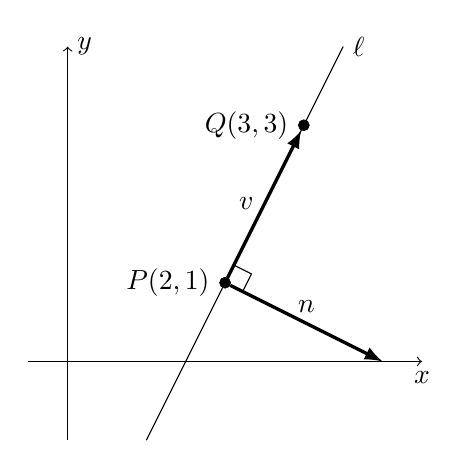
\begin{tikzpicture}[
	point/.style={circle,draw,very thin,fill,inner sep=0pt,minimum size=4pt},
	vector/.style={-latex,very thick},
	% scale=0.75
]
	\draw[->] (-0.5,0) to (4.5,0) node[below] {$x$};
	\draw[->] (0,-1) to (0,4) node[right] {$y$};

	% slope: over 1 up 2
	\draw (1,-1) to (3.5,4) node[right] {$\ell$};

	\node[point] at (2,1) (p) [label=left:{$P(2,1)$}] {};
	\node[point] at (3,3) (q) [label=left:{$Q(3,3)$}] {};

	\draw[vector] (p) to node[left] {$\uvec{v}$} (q);

	\draw[vector] (p) to node[above] {$\uvec{n}$} ++(2,-1);

	% perp symbol
	\begin{scope}[xshift=2cm,yshift=1cm]
		\draw[thin,rotate=-26.565] (0.25,0) to (0.25,0.25) to (0,0.25);
	\end{scope}

\end{tikzpicture}
